% !TEX root = paper.tex
% =============================================================
% RAR — Evaluation Section Scaffold (v0)
% Source-of-truth: project_context.md (Binding constraints).
% Stage 3 of paper-writing skill. Draft 0 intro frozen 2026-07-09.
% Last updated: 2026-07-09
%
% Conventions
%   - KDD venue: integrated related work, colon-style subtitles, no \smartparagraph.
%   - Headings are claims. Topic sentences assert claims.
%   - Every subsection ends with a "Takeaway." paragraph.
%   - Main tables have been populated from the organized results.
%   - Reference metadata remains to be finalized before submission.
%   - Mechanism: SOFT routing via reconstruction-temperature-weighted dual heads.
%     Do not describe RAR as assigning each sample to a single head.
% =============================================================

\section{Experiments}\label{sec:eval}
% Section opener: claim-first. The headline number lives in the section heading.
% Each subsection below tests a specific claim from the introduction (C1--C4).
% Setup first (§4.1), then head-to-head (§4.2 and §4.3 split by Principle 9),
% then ablations (§4.4), optional robustness (§4.5), then honest disaggregation (§4.6).

% -----------------------------------------------------------------
% §4.1 Setup Anchoring  -- full prose per the deferred-action contract
% -----------------------------------------------------------------
\subsection{Experimental Setup}

We evaluate RAR on six public encrypted-traffic datasets that span several application and threat surfaces: mobile app traffic (NUDT-Mobile), DNS-over-HTTPS (CIC-DoHBrw), IoT attack traffic (CIC-IoT2023), TLS~1.3 application traffic (CSTNET-TLS1.3), Tor traffic (ISCX-Tor), and web application traffic (EBSNN-WebApp). Table~\ref{tab:datasets} reports their sizes and class counts.

\begin{table}[t]
\caption{Six encrypted-traffic datasets used in evaluation.}
\label{tab:datasets}
\centering
\footnotesize
\begin{tabular}{p{2.4cm}llrr}
\toprule
Dataset & Domain & Public & \#Cls & \#Flows \\
\midrule
NUDT-Mobile      & Mobile app     & Yes & 300 & 496086 \\
CIC-DoHBrw       & DNS-over-HTTPS & Yes & 6 & 49777 \\
CIC-IoT2023      & IoT attack     & Yes & 22 & 26413 \\
CSTNET-TLS1.3    & TLS 1.3 app    & Yes & 120 & 43243 \\
ISCX-Tor         & Tor            & Yes & 26 & 8518 \\
EBSNN-WebApp     & Web app        & Yes & 48 & 15336 \\
\bottomrule
\end{tabular}
\end{table}

We compare RAR against two baseline groups. \emph{Group A} holds the encoder fixed at ET-BERT~\cite{lin2022etbert} and varies the CIL strategy: Learning without Forgetting (LwF)~\cite{li2017lwf}, iCaRL~\cite{rebuffi2017icarl}, BiC~\cite{wu2019bic}, DER~\cite{yan2021der}, Adapter~\cite{houlsby2019adapter}, Fine-tune, and an ET-BERT adaptation of MORE~\cite{kim2022more}. \emph{Group B} holds the naive CIL setup fixed and varies the traffic-classification backbone across nine models: AppScanner, ETC-PS, FlowLens, CNN-based, CNN-emb, EBSNN, FS-Net, GraphDApp, and MM4flow. RAR with ET-BERT is included as a reference rather than counted as a tenth backbone baseline. Group~A compares routing with both classical CIL strategies and a closely related OOD-replay multi-head method on a fixed encoder; Group~B tests whether naive incremental forgetting persists across encoder choices.

\begin{table}[t]
\caption{Baseline groups.}
\label{tab:baselines}
\centering
\small
\begin{tabular}{lll}
\toprule
Group & Variable held fixed & Baselines \\
\midrule
A & ET-BERT encoder & LwF, iCaRL, BiC, DER, Adapter,\\
  &                   & Fine-tune, MORE \\
B & Replay + head expansion & AppScanner, ETC-PS, FlowLens,\\
  &                        & CNN-based, CNN-emb, EBSNN,\\
  &                        & FS-Net, GraphDApp, MM4flow \\
\bottomrule
\end{tabular}
\end{table}

Five metrics isolate the quantity each claim depends on. \emph{old-before} measures accuracy on old classes after head expansion and \emph{before} training on the new step. \emph{old-after} measures accuracy on old classes after training on the new step. \emph{new-after-train} measures accuracy on the new classes after the new step. \emph{mix} reports combined accuracy on old plus new classes after the new step. \emph{forgetting} equals \emph{old-before} minus \emph{old-after} and isolates training-induced forgetting, so the head-expansion drop alone does not contribute.

We report forgetting and mix as the headline pair: forgetting measures old-class retention after incremental training, and mix captures the joint old/new accuracy that operators observe. Together they evaluate the two outcomes that reconstruction-conditioned balancing is designed to improve.

All experiments share one training and evaluation pipeline. The encoder remains frozen. During an increment, the inherited old path and the fitted reconstructor are frozen; the adapter, new-class pathway, and calibration scalars are trainable. The calibration scalars are subsequently refined on a mixed validation set.

Before incremental training, we repartition the provided new-class evaluation split using a fixed random seed (42), reserving 10\% for validation and the remaining 90\% for held-out testing. The validation and held-out test subsets are disjoint, and the old-class test split is evaluated independently.

The main comparison uses a two-stage protocol: a base stage trains the initial head on the first half of classes, and one incremental stage learns the remaining classes with a fixed replay buffer. Section~\ref{sec:eval-buffer} additionally evaluates the recursive five-increment protocol defined in Section~\ref{sec:multistep}.

% -----------------------------------------------------------------
% §4.2 Group A -- RAR vs classical CIL strategies. Topic sentences + table + Takeaway.
% -----------------------------------------------------------------
\subsection{Comparison with CIL Strategies}
% Tests C1: reconstruction-aware old/new balancing.
% Headline: forgetting cut by 35.5%--67.5% (vs Adapter, mean 47.8%); mix raised by up to 11.7 pp.

% Topic sentence 1: claim
Against classical CIL strategies on a fixed ET-BERT encoder, RAR cuts forgetting by an average of 47.8\% (range 35.5\%--67.5\%) across six datasets and raises mixed-class accuracy by up to 11.7 percentage points over the strongest evaluated baseline (Adapter).

% Topic sentence 2: pattern
Replay-based methods (DER, iCaRL) outperform uniform distillation (LwF) under encrypted traffic, yet both still forget more than RAR on every dataset.

% Topic sentence 3: fine-tuning reference
Fine-tune, which omits all anti-forgetting mechanisms, provides a naive incremental reference. RAR reduces forgetting by 35.5\%--67.5\% relative to the strongest evaluated baseline (Adapter) on every dataset.

% Topic sentence 4: pattern citation (Principle 14)
The consistent gains are compatible with the intended effect of reconstruction-error routing: adapting preservation and acquisition signals to each flow rather than applying a uniform balance.

% Topic sentence 5: figure/table reference
\begin{table*}[t]
\caption{Forgetting ($F\!\downarrow$, lower is better) and mixed-class accuracy ($M\!\uparrow$, higher is better). Mean over 3 seeds; \emph{TBD} marks runs in progress.}
\label{tab:eval-a}
\centering
\small
\setlength{\tabcolsep}{6pt}
\renewcommand{\arraystretch}{1.05}

\begin{tabular}{p{1.8cm}|
>{\centering\arraybackslash}p{0.55cm}@{\hspace{8pt}}
>{\centering\arraybackslash}p{0.55cm}|
>{\centering\arraybackslash}p{0.55cm}@{\hspace{8pt}}
>{\centering\arraybackslash}p{0.55cm}|
>{\centering\arraybackslash}p{0.55cm}@{\hspace{8pt}}
>{\centering\arraybackslash}p{0.55cm}|
>{\centering\arraybackslash}p{0.55cm}@{\hspace{8pt}}
>{\centering\arraybackslash}p{0.55cm}|
>{\centering\arraybackslash}p{0.55cm}@{\hspace{8pt}}
>{\centering\arraybackslash}p{0.55cm}|
>{\centering\arraybackslash}p{0.55cm}@{\hspace{8pt}}
>{\centering\arraybackslash}p{0.55cm}
}
\toprule

& \multicolumn{12}{c}{Dataset} \\
\cmidrule(lr){2-13}
Method
& \multicolumn{2}{c|}{NUDT}
& \multicolumn{2}{c|}{DoH}
& \multicolumn{2}{c|}{IoT}
& \multicolumn{2}{c|}{TLS}
& \multicolumn{2}{c|}{Tor}
& \multicolumn{2}{c}{Web} \\

& $F\!\downarrow$
& $M\!\uparrow$
& $F\!\downarrow$
& $M\!\uparrow$
& $F\!\downarrow$
& $M\!\uparrow$
& $F\!\downarrow$
& $M\!\uparrow$
& $F\!\downarrow$
& $M\!\uparrow$
& $F\!\downarrow$
& $M\!\uparrow$ \\

\midrule
Fine-tune & 95.40 & 33.71 & 91.58 & 36.74 & 88.52 & 11.17 & 90.99 & 46.52 & 86.25 & 41.31 & 86.01 & 43.19 \\
LwF~\cite{li2017lwf} & 61.03 & 55.91 & 88.91 & 36.75 & 52.58 & 43.53 & 56.21 & 65.66 & 96.37 & 34.72 & 78.11 & 48.20 \\
iCaRL~\cite{rebuffi2017icarl} & 25.15 & 81.66 & 33.87 & 73.25 & 12.39 & 79.47 & 28.87 & 80.83 & 73.60 & 69.90 & 37.77 & 73.97 \\
BiC~\cite{wu2019bic} & 24.78 & 79.48 & 33.87 & 73.25 & 11.68 & 80.09 & 28.94 & 80.65 & 84.87 & 42.21 & 38.15 & 73.61 \\
DER~\cite{yan2021der} & 12.64 & 86.15 & 33.92 & 73.19 & 11.33 & 79.37 & 16.85 & 85.11 & 77.28 & 46.83 & 17.89 & 84.78 \\
Adapter~\cite{houlsby2019adapter} & 12.79 & 86.86 & 33.86 & 73.26 & 9.22 & 82.12 & 16.40 & 87.20 & 13.11 & 89.16 & 13.98 & 88.69 \\
MORE~\cite{kim2022more}
& \textit{TBD} & \textit{TBD}
& \textit{TBD} & \textit{TBD}
& \textit{TBD} & \textit{TBD}
& \textit{TBD} & \textit{TBD}
& \textit{TBD} & \textit{TBD}
& \textit{TBD} & \textit{TBD} \\

\midrule

RAR (ours)
& \textbf{6.65} & \textbf{90.12}
& \textbf{11.00} & \textbf{84.93}
& \textbf{4.82} & \textbf{86.05}
& \textbf{8.49} & \textbf{91.70}
& \textbf{8.45} & \textbf{91.94}
& \textbf{8.37} & \textbf{92.30} \\

\bottomrule
\end{tabular}
\end{table*}

% -----------------------------------------------------------------
% §4.3 Group B -- RAR vs 9 traffic-classification backbones.
% -----------------------------------------------------------------
\subsection{Backbone Study}\label{sec:eval-bgroup}
% Tests whether the forgetting problem depends on the encoder. Drill-down on NUDT-Mobile; Group A generalizes across the six datasets.

% Topic sentence 1: claim
On NUDT-Mobile, naive incremental training forgets across all nine traffic-classification backbones, which isolates the forgetting problem from the encoder choice.

% Topic sentence 2: pattern
Forgetting spans 13.3\%--58.4\% across the nine naive backbones despite their different representation architectures. Even the lowest-forgetting naive backbone (GraphDApp, 13.3\%) forgets more than twice as much as RAR's 6.65\% under the evaluated setup.

% Topic sentence 3: implication for encoder choice
Changing the encoder alone does not eliminate the old-class accuracy loss under naive incremental training. RAR yields lower forgetting than every naive-backbone configuration in this study (6.65\% vs 13.3\% for the lowest-forgetting configuration, GraphDApp).

% Topic sentence 4: figure/table reference
Table~\ref{tab:eval-b-forgetting} reports the naive-incremental forgetting rate and mix accuracy for each of the nine backbones on NUDT-Mobile, with RAR shown for contrast.

\begin{table}[t]
\caption{Naive-incremental forgetting and mix (\%) on NUDT-Mobile.}
\label{tab:eval-b-forgetting}
\centering
\small
\begin{tabular}{lcc}
\toprule
Backbone & Forgetting (\%) & Mix (\%) \\
\midrule
AppScanner          & 58.37 & 49.30 \\
ETC-PS              & 56.63 & 47.99 \\
FlowLens            & 56.99 & 45.69 \\
CNN-based           & 44.10 & 58.66 \\
CNN-emb             & 41.27 & 63.89 \\
EBSNN               & 30.81 & 73.37 \\
FS-Net              & 23.35 & 74.70 \\
GraphDApp           & 13.26 & 55.54 \\
MM4flow             & 22.45 & 81.61 \\
\midrule
RAR (ours)          & 6.65 & 90.12 \\
\bottomrule
\end{tabular}
\end{table}

% -----------------------------------------------------------------
% §4.4 Ablations
% -----------------------------------------------------------------
\subsection{Ablation Study}
% Tests C2, C3, and C1 attribution. E8 reports the design knob (Q28).

We ablate RAR's three principal components and its use of soft routing. \emph{w/o flow-aware routing} removes the complete per-flow reconstruction-aware routing mechanism to measure its overall contribution. \emph{w/o dual-head} replaces the old/new paths with a single expanded classifier, and \emph{w/o calibration} omits post-training logit alignment. \emph{hard routing} retains the reconstructor, dual paths, objectives, and calibration, but replaces the continuous scores with $s_{\mathrm{old}}(x)=\mathbf{1}\{e(x)\leq\theta\}$ and $s_{\mathrm{new}}(x)=1-s_{\mathrm{old}}(x)$ for binary loss weighting and single-path inference. It isolates the benefit of continuous weighting from that of flow-level old/new decisions.

\begin{table}[t]
\caption{Ablation results on NUDT-Mobile.}
\label{tab:ablation}
\centering
\small
\begin{tabular}{lcc}
\toprule
Variant & Forgetting (\%) & Mix (\%) \\
\midrule
w/o flow-aware routing & 12.43 & 87.29 \\
w/o dual-head     & 11.14 & 80.35 \\
w/o calibration   & 10.06 & 87.82 \\
hard routing      & 10.42 & 80.13 \\
\midrule
RAR (full)        & 6.65  & 90.12 \\
\bottomrule
\end{tabular}
\end{table}

Removing flow-aware routing nearly doubles forgetting, from 6.65\% to 12.43\%, demonstrating the overall effectiveness of per-flow reconstruction-aware adaptation. A single expanded head raises forgetting to 11.14\% and lowers mix from 90.12\% to 80.35\%, while removing calibration raises forgetting to 10.06\% and lowers mix to 87.82\%; these results support old/new path separation and logit alignment, respectively. Hard routing also degrades forgetting to 10.42\% and mix to 80.13\%. Its 9.99\,pp mix drop shows the cost of discarding one path after a binary decision, supporting continuous soft integration for flows near the reconstruction boundary.

% E8 -- tau sensitivity (the Q28 design knob)
\paragraph{Reconstruction temperature $\tau$ (design knob).}\label{sec:eval-ablation-tau}
Figure~\ref{fig:tau-sensitivity} reports forgetting and mix on CSTNET-TLS1.3 as $\tau$ sweeps from 0.25 (near-deterministic head selection) to 4.0 (near-uniform fusion). Forgetting drops from 9.71\% at $\tau{=}0.25$ to 7.78\% at $\tau{=}4.0$, and mix rises from 91.03\% to 92.06\%. The curve flattens after $\tau{=}1.0$: the difference between $\tau{=}1.0$ and $\tau{=}4.0$ is under 0.2\,pp on both metrics. RAR therefore exposes a tunable knob that converges quickly; the operator can fix $\tau{=}1.0$ (the fitted value) without further tuning.

\begin{figure}[t]
\centering
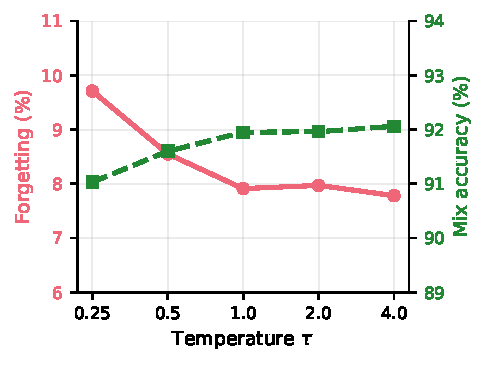
\includegraphics[width=\linewidth]{figures/tau_sensitivity.pdf}
\caption{Forgetting and mix as a function of $\tau$, on CSTNET-TLS1.3.}
\label{fig:tau-sensitivity}
\Description{Dual-axis line plot of forgetting rate and mix accuracy against temperature tau on CSTNET-TLS1.3. Red line with circles shows forgetting decreasing from 9.71 to 7.78 percent. Green dashed line with squares shows mix accuracy rising from 91.03 to 92.06 percent. The curves flatten after tau equals 1.0, indicating the sweet spot.}
\end{figure}

% -----------------------------------------------------------------
% §4.5 Robustness
% -----------------------------------------------------------------
\subsection{Robustness}\label{sec:eval-buffer}
% T = 5 steps. Buffer sweep = {5, 10, 20, 50} per class. CSTNET-TLS1.3.

% Topic sentence 1: claim
Over $T$ incremental steps and a range of replay-buffer sizes, RAR maintains its lead over Adapter, the strongest evaluated classical CIL baseline overall.

We select Adapter for these robustness experiments because it provides the strongest overall performance among the evaluated classical CIL baselines in Table~\ref{tab:eval-a}, while allowing the same frozen ET-BERT encoder, data splits, replay protocol, and memory budgets as RAR. This controlled comparison tests whether RAR's advantage persists across incremental steps and constrained replay budgets; the broader method comparison remains in Table~\ref{tab:eval-a}.

% Topic sentence 2: per-step pattern
We split the 40 new classes of CSTNET-TLS1.3 into $T=5$ steps of 8 classes each. Fine-tune collapses from 75.6\% to 22.0\% mix accuracy after five steps. Adapter degrades from 91.3\% to 74.8\%. RAR drops only from 93.4\% to 84.6\%, widening its lead over Adapter from 2.1\,pp at $T{=}1$ to 9.8\,pp at $T{=}5$.

% Topic sentence 3: buffer pattern
Across all evaluated memory ratios, RAR exhibits lower forgetting than Adapter. At the smallest ratio of 0.005, RAR records 11.82\% forgetting, compared with 22.70\% for Adapter. Increasing the ratio to 0.05 reduces the endpoint values to 5.98\% and 7.97\%, respectively, although the intermediate RAR results are not strictly monotonic. Notably, RAR at ratio 0.005 achieves forgetting comparable to Adapter at a four-times-larger ratio of 0.02 (11.82\% versus 11.70\%).

% Topic sentence 4: figure/table reference
Figure~\ref{fig:robustness} reports the per-step accuracy and buffer sensitivity on CSTNET-TLS1.3.

\begin{figure}[t]
\centering
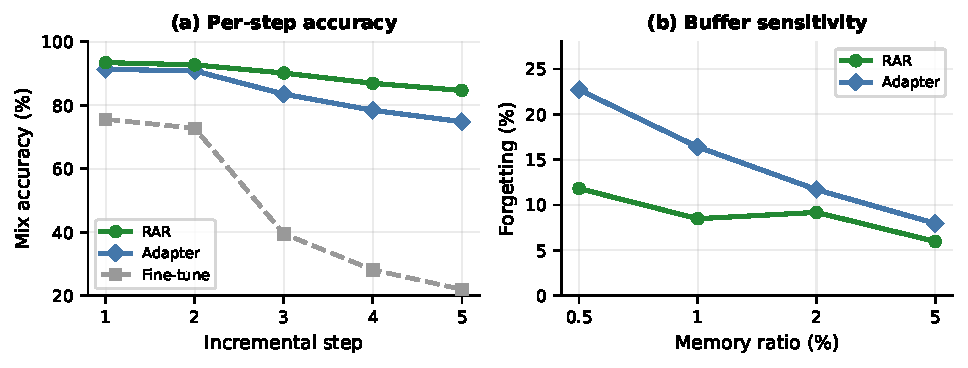
\includegraphics[width=\linewidth]{figures/robustness.pdf}
\caption{Robustness on CSTNET-TLS1.3: (a) per-step mix accuracy over $T=5$ steps, and (b) forgetting as a function of memory ratio.}
\label{fig:robustness}
\Description{Two-panel figure. Left: line plot of per-step mix accuracy on CSTNET-TLS1.3 over five incremental steps with RAR, Adapter, and Fine-tune. Right: line plot of forgetting rate against memory ratio for RAR and Adapter. RAR has higher per-step mix accuracy and lower forgetting at every evaluated memory ratio.}
\end{figure}
